% ------------------------- MAIN TASK ---------------------------------
\section{Développement du PCB}

\subsection{Bill of materials} \label{ssec:BOM}
{
	La BOM complète est disponible dans les répertoires du projet, voici un extrait des prix des composants importants :
	
	\begin{figure}[h]
		\centering
		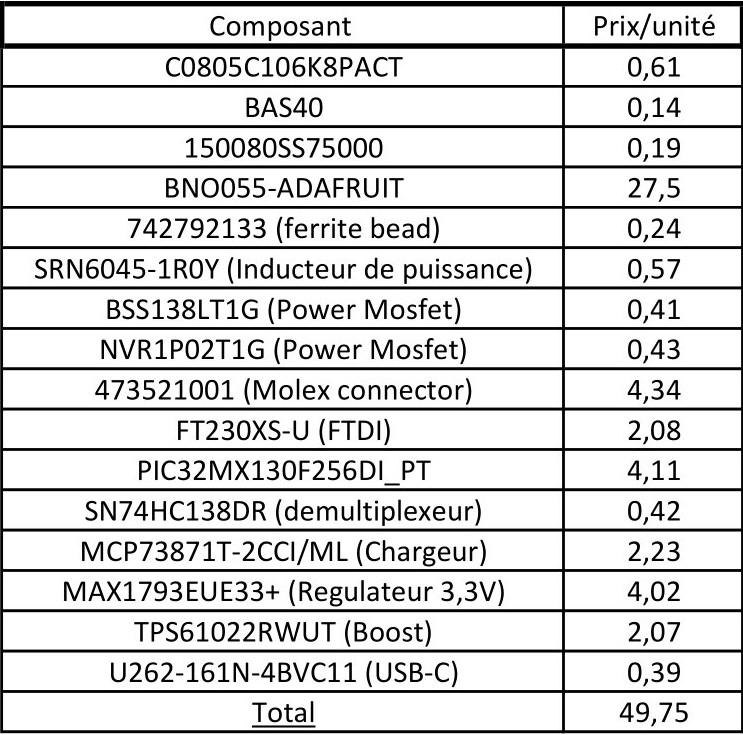
\includegraphics[width=0.7\linewidth]{Figures/Prix_Composants}
		\caption{Prix des composants}
		\label{fig:prixcomposants}
	\end{figure}
	
}
\clearpage

\subsection{Mécanique du projet} \label{ssec:mechProjet}
{
	Afin d'installer le PCB dans le boitier de la lampe, les deux tiges internes du boitier peuvent avec des attaches servir de support. Pour se faire, imprimer une pièce a visser en 3d ou en utilisant simplement des brides, pourrait permettre de maintenir la carte dans le boitier. Il faudra donc mettre des trous dans le PCB pour permettre des visses ou des brides.
	
	
	\subsubsection{Considérations mécaniques} \label{ssec:RestrictionMech}
	\paragraph{Tige conductrice :} Sachant que les tiges de support de la lampe sont conductrices, il faut donc prévoir une zone sans composant, sans cuivre apparent et si possible sans pistes sur les bords de la couche \textit{bottom}.
	\paragraph{Carte SD : } La carte SD requiert un support relativement grand et un espace doit être prévu pour pouvoir insérer/retirer la carte facilement et sans qu'elle dépasse trop du PCB.
	\paragraph{Centra inertielle :} La centrale inertielle, se connecte via des bergs femelles et vas par conséquent prendre de la place en hauteur, ce qui doit être considéré.
	\paragraph{Slot MIKROE :} Un slot mikroe est présent dans le projet et pour être implémenté, vas requérir un allongement mécanique du bouton de la lampe, pour gagner de la place. Cette pièce doit être produite et usinée, car elle requiert d'être étanche. 
	\paragraph{LED RGB :} La LED en bout du PCB peut exploiter le réfracteur déjà présent de la lampe.
	\paragraph{Connecteur USB :} Pour charger l'appareil, un port USB devrait être disponible au bord du PCB.
}
\clearpage

\subsection{Placement des composants} \label{ssec:placementComp}
{
\paragraph{Alimentation :}
\begin{figure}[h]
	\centering
	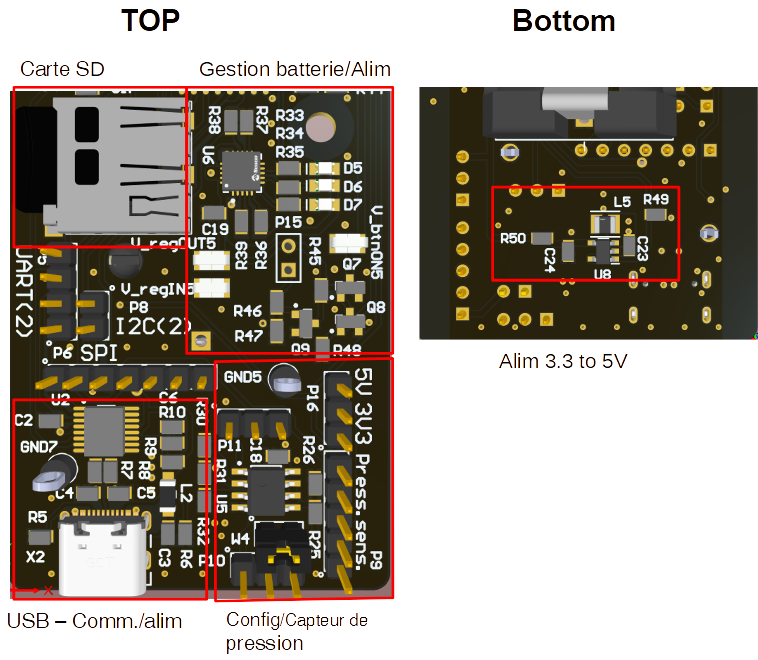
\includegraphics[width=0.9\linewidth]{Figures/BasPCB}
	\caption{Placement alimentations}
	\label{fig:baspcb}
\end{figure}

J'ai décidé de placer en bas du PCB les parties d'alimentations du projet. Cette zone comporte :

% Please add the following required packages to your document preamble:
% \usepackage{graphicx}
\begin{table}[h]
	\centering
	\resizebox{\textwidth}{!}{%
		\begin{tabular}{|c|l|l|}
			\hline
			Composant &
			\multicolumn{1}{c|}{Detail} &
			\multicolumn{1}{c|}{Justification} \\ \hline
			USB &
			FTDI, piste 5V, pistes différentiels &
			Bord du PCB pour cablage ergonomique \\ \hline
			Capteur de pression &
			\begin{tabular}[c]{@{}l@{}}Connecteur, Jumper choix alim,\\ Choix mode (courant,tension,i2c)\end{tabular} &
			\begin{tabular}[c]{@{}l@{}}Capteur de pression proche du bord\\ branchement plus simple\end{tabular} \\ \hline
			Carte SD &
			Condos de découplages, pistes SPI &
			Plus grand consommateur \\ \hline
			Gestion batterie &
			\begin{tabular}[c]{@{}l@{}}Régulateur de charge, bouton ON/OFF,\\ régulateur 3.3V\end{tabular} &
			Zone dédiée, proche de la batterie \\ \hline
			Boost 5V (bottom) &
			Circuit de boost 3.3-5V &
			\begin{tabular}[c]{@{}l@{}}Isolé, loin des petits signaux (bruit).\\ Proche du capteur de pression (5V)\end{tabular} \\ \hline
		\end{tabular}%
	}
	\caption{Composants de la zone et justification}
	\label{tab:PlacementBas}
\end{table}
\clearpage

\begin{figure}[h]
	\centering
	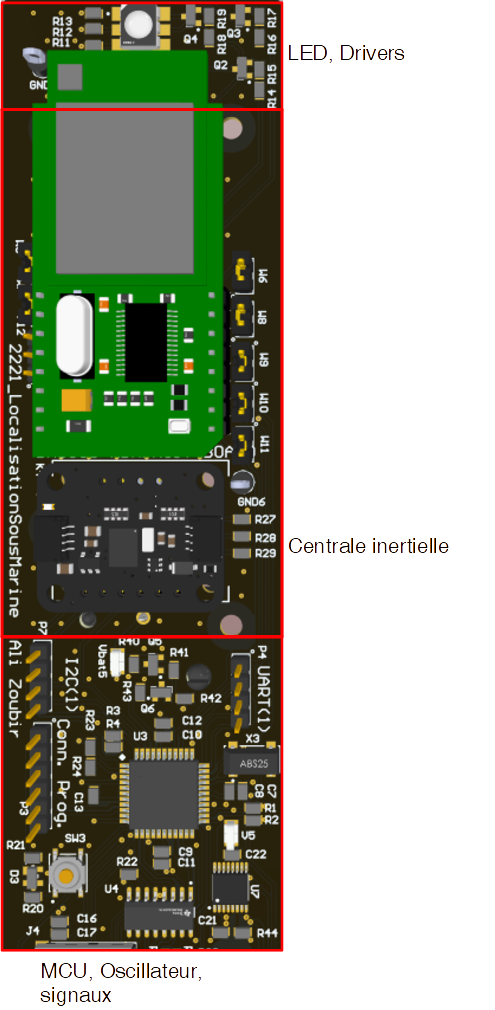
\includegraphics[width=0.56\linewidth]{Figures/hautPCB}
	\caption{Placement signaux}
	\label{fig:hautpcb}
\end{figure}

Le microcontrôleur est plus ou moins centrée par rapport aux différents périphériques, afin de minimiser la longueur des pistes des petits signaux. Il y a un bouton de reset, un multiplexeur et un oscillateur externe, au plus proche du MCU.
}
\clearpage

\subsection{Routage} \label{ssec:routage}
{
	\begin{figure}[h]
		\centering
		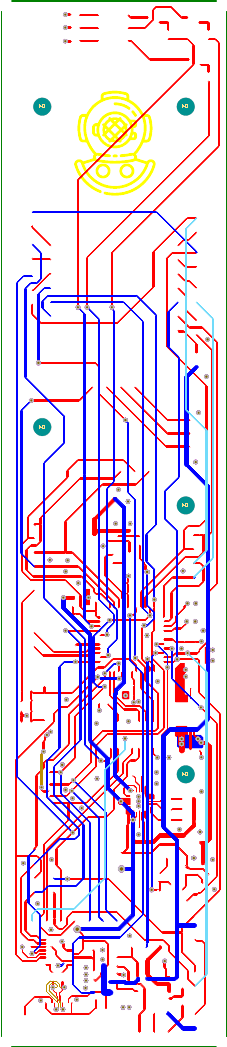
\includegraphics[height=0.615\pageheight]{Figures/Pistes}
		\caption{Pistes du PCB}
		\label{fig:pistes}
	\end{figure}
	
}
\clearpage

\subsection{Points d'améliorations} \label{ssec:pointAmel}
{}
\clearpage

\subsection{Conclusion du projet} \label{ssec:conclusionG}
{}
\clearpage